\documentclass[12pt]{article}

% Packages for formatting and math
\usepackage{amsmath, amsthm, amssymb}
\usepackage{cite}
\usepackage{geometry}
\usepackage{csquotes}
\geometry{a4paper, margin=2.5cm}

\usepackage{parskip}
\usepackage{amssymb}
\usepackage{tikz}
\usepackage{amsfonts}
\usepackage{enumitem}
\usepackage[colorinlistoftodos,prependcaption,textsize=tiny]{todonotes}
\usepackage{wrapfig}

% Format bibliography links correctly
\usepackage[hidelinks]{hyperref}
\usepackage[T1]{fontenc}
\usepackage{mathtools}

% Theorem and Proof setup
\newtheorem{theorem}{Theorem}
\newtheorem{lemma}{Lemma}
\newtheorem{definition}{Definition}

% Title Section
\title{MATD02 - Exploration of Finite Geometry }
\author{Danielle Voznyy}
\date{}

\begin{document}

    \maketitle

    \begin{abstract}
        We explore finite geometries through a synthetic point of view.
        Starting with axioms, we define finite projective spaces and planes.
        We discuss the concepts of order and dimension in these spaces,
        specifically how dimension in projective spaces can be described without a coordinate system.
        Finally, we discuss an open conjecture about the order of finite planes.
    \end{abstract}


    \section{Introduction}

    Finite geometries provide a good starting point to axiomatic, sometimes called synthetic, definitions of geometries.
    We can visualize finite geometries with as little as 7 points and lines and use them to explore abstract concepts.
    We'll begin by describing finite geometries using two sets and the set containment relation.\footnote{
        Both the definition for geometries and projective spaces are modified from \cite[p.~1,7]{beutelspacher_projective_1998},
        which uses an arbitrary symmetric and reflexive relation.
        We opt for set containment for its familiarity.}

    \begin{definition}
        Let $P$ be nonempty a finite set and $\mathcal{L} \subseteq \mathcal{P}(P)$, be a nonempty subset of the power set of $P$,
        then $(P, \mathcal{L})$ is finite a geometry.

        We call an element of $P$ a point in our space, and an element of $\mathcal{L}$ a line.
        We say a point $p$ is on a line $L$ when $p \in L$ and lines $L_1, L_2$ intersect when $L_1 \cap L_2 \neq \emptyset$.
    \end{definition}

    We can now categorize these spaces using axioms, starting with planes.
    Two broad types of plane geometries come from a similar set of axioms which differ in the existence of parallel lines.
    Affine geometry, where parallel lines exist, and projective geometry, where they do not.
    As it turns out, these are quite similar despite projective geometry being simpler to work with.

    We start by defining projective spaces and planes axiomatically:

    \begin{definition}
        A projective space is a geometry such that,
        \begin{itemize}[noitemsep]
            \item A1 - For distinct points $p, q$, there is exactly one line $L$ such that $\{p,q\} \subseteq L$.
            We call it the line containing $p, q$, or just the line $pq$.
            \item A2 - Given distinct points $a,b,c,d$, if $ab$ intersects $cd$, then $ac$ intersects $bd$
            \item A3 - Any line contains at least 3 elements.
            \item A4 - We call this projective space a projective plane if any two lines have at least one point in common, i.e. they intersect
            \item S1 - To avoid simple cases, we add that at least two lines (and thus points) exist.
        \end{itemize}
    \end{definition}



%   From: https://tex.stackexchange.com/questions/208894/how-might-i-typeset-the-fano-plane-in-latex
%    \begin{figure}[h]
    \begin{wrapfigure}{r}{0.25\textwidth}
        \centering
        \label{fig:fano_plane}
        \tikz[every node/.style={circle, fill, scale=0.5}]
        \draw circle [radius=1] (90:2) -- (210:2) -- (330:2) -- cycle (0,0) node {}
        \foreach \i in {90,210,330}{ (\i:2) node {} -- (\i+180:1) node {} };
    \end{wrapfigure}

    The Fano plane, shown to the right, is an example of such a projective plane,
    in fact it is the smallest projective plane, containing 7 points and 7 lines.

    It's fairly routine work to show the set of points and lines shown do in fact satisfy our earlier axioms,
    however more interesting is that this plane has the same number of points and lines, and all lines contain 3 points.
    Does this generalize to all projective spaces?


    \section{Order of finite projective spaces}

    In fact, it does generalize, we call the first concept duality,
    in which theorems about lines on a projective plane also have duals regarding points (and vice-versa).
    In finite projective spaces, the second gives rise to a concept of order\cite[p. 24]{beutelspacher_projective_1998}.

    \begin{theorem}
        Given a finite projective space $(P, \mathcal{L})$, there exists a positive integer $q$ such that any line in $\mathcal{L}$ contains exactly $q+1$ elements.
        We call $q$ the order of this space.
    \end{theorem}

    \begin{proof}
        Given any two lines $L_1, L_2$, we'll argue there exists a bijection $\phi: L_1 \rightarrow L_2$,
        and thus all lines have the same number of elements.
        When our set of points is finite, this implies the existence of an integer order.
        If $L_1 = L_2$ we are done, so we consider distinct lines.

        \underline{Case 1}: $L_1$ intersects $L_2$.
        Then $\{a, b\} \subseteq L_1$ and $\{a, c\} \subseteq L_2$ for some points $a,b,c$,
        since by A3 both lines contain at least 3 distinct points and by supposition we have at least one shared point.
        By A3 again, line $bc$ must contain another point, name it $p$, moreover $p \notin L_1, L_2$,
        otherwise $L_1 = L_2$ by A1, the uniqueness of lines through points.

        Then given any other point $x \in L_1$, consider the line $xp$.
        We'll show this must intersect $L_2$ and call the intersection point $\phi(x)$.

        \begin{figure}[h]
            \centering
            \begin{tikzpicture}
                % Draw the lines
                \draw[thick] (-2,0) -- (3,1) node[right] {$L_1$};
                \draw[thick] (-2,0) -- (3,-1) node[right] {$L_2$};
                % Draw the intersection point
                \fill (-2,0) circle (2pt) node[below] {$a$};
                % Label points on L1
                \fill (2,0.8) circle (2pt) node[above] {$b$};
                \fill (0,0.4) circle (2pt) node[above] {$x$};
                % Label points on L2
                \fill (2,-0.8) circle (2pt) node[below] {$\phi(x)$};
                \fill (0,-0.4) circle (2pt) node[below] {$c$};
                % Draw intersecting lines
                \draw[thick] (2,-0.8) -- (0,0.4)
                \draw[thick] (2,0.8) -- (0,-0.4)
                \fill (0.7,0) circle (2pt) node[below] {$p$};
            \end{tikzpicture}
%            \caption{Illustration of our points and lines}
            \label{fig:intersecting_lines}
        \end{figure}
        By A2: If $xa$ intersects $pc$, then $xp$ intersects $ac$.
        We have $pc=bc$ and $xa = ab$ by A1, so both lines contain $b$ and thus intersect.
        So $xp$ intersects $ac$.
        We define the function $\phi(x)$ with domain $L_1$ as follows:

        \[
            \phi(x) =
            \begin{cases}
                xp \cap L_2 & \text{if } x \neq a \\
                a & \text{if } x = a
            \end{cases}
        \]

        Let $x_2\in L_1$ be distinct from $a, x$.
        Then $\phi(x_2) \neq \phi(x)$,
        since both pass through p and otherwise by A1 we would have $x = x_2$.
        Using the same logic as earlier, for $y \in L_2$ distinct from $a$, the line $yp$ intersects $L_1$ at a point $x$ such that $\phi(x)=y$.
        Finally, since $\phi$ also maps $a \in L_1$ to $a \in L_2$, $\phi$ is a bijection from $L_1$ to $L_2$.

        \underline{Case 2}: $L_1$ does not intersect $L_2$.
        Let $x \in L_1, y \in L_2$, then the line $L_3 \coloneqq xy$ intersects with both $L_1$ and $L_2$, so from case 1 we have bijections
        $\phi_1: L_1 \rightarrow L_3$ and $\phi_2: L_3 \rightarrow L_2$, and thus a bijection $\phi_1 \circ \phi_2: L_1 \rightarrow L_2$.
    \end{proof}


    \section{Dimension of finite projective spaces}

    The use of the term plane for our extra axiom\textemdash stating any two lines must intersect\textemdash seems connected to a two-dimensional space.
    We might now wonder what this axiom actually does, and what the idea of dimension even means for the abstract sets we used.

    In fact, when looking at projective geometry through the lens of infinite fields like $\mathbb{R}$,
    we get a definition of projective spaces from one-dimensional vector subspaces of a vector space like $\mathbb{R}^n$\cite{weisstein_projective_nodate}.
    Here, our dimension comes from a concept of coordinates in the underlying vector space, i.e.\ its basis.
    Working purely from axioms we don't have such an obvious idea of dimension.
    We can, however, generalize concepts from vector spaces to get the following definitions.\footnote{
        The two definitions come from Wikipedia \cite{noauthor_projective_2024},
        I could not find a text referencing them exactly, my assumption is something cited nearby states them in a modified form.
        Nevertheless, I found them fascinating as a demonstration of dimension in an abstract context.
    }

    \begin{definition}
        A subspace of a projective space $(P, \mathcal{L})$ is a projective space of points $X \subseteq P$ and lines $\mathcal{Y} \subseteq \mathcal{L}$,
        such that any line containing two points of X is a subset of X (that is, completely contained in X).
        The full space and the empty space are always subspaces.
    \end{definition}

    \begin{definition}
        The geometric dimension of the space $(P, \mathcal{L})$ is said to be n if that is the largest number for which there is a strictly ascending chain of subspaces of this form:
        \begin{center}
            $\emptyset = X_{-1}\subset X_{0}\subset \cdots X_{n}=P.$
        \end{center}
    \end{definition}

    \begin{theorem}
        Projective planes are projective spaces of dimension 2.
    \end{theorem}

    \begin{proof}
        Let $P$ be the set of points in our plane, noting $|P|\geq 2$ by S1.

        \underline{Part 1}: \textit{The dimension of our plane must be at least 2.}

        Consider any point $a \in P$, $\{ a \}$ is a subspace of $P$ vacuously since it doesn't contain two points.
        Now, given any other point $b$, $ab$ is the only line that passes through two points of $ab$ by A1.
        So $ab$ is a subspace since $ab \subseteq ab$.
        Finally, $P$ has at least two lines by S1, so $ab \subset P$.
        So we have a chain of subspaces $\emptyset \subset \{a\} \subset ab \subset P$, thus our geometric dimension is at least 2.

        \underline{Part 2}: \textit{The dimension of our plane must be at most 2.}

        In a maximal chain of subspaces, any subspace $X_i$ must have that there does not exist a subspace $X$ for which $X_{i-1} \subset X \subset X_i$.
        Since any nonempty subspace $X$ must contain a point $a$ and $\{a\}$ is a subspace (as shown earlier),
        with no sets existing between $\emptyset$ and $\{a\}$, we must have in our chain that $X_0 = \{a\}$.

        Similarly, since $X_0 \subset X_1$, $X_1$ contains at least another point $b$, and again the line $ab$ is a subspace as shown earlier.
        Any strict subset of $ab \neq \emptyset, \{a\}$ would not contain the line $ab$ in full and thus cannot be a subspace.
        So it must be that $X_1 = ab$.

        Now, since $X_1 \subset X_2$, we must have a distinct $c \in X_2$ such that $c \notin X_2 = ab$.
        So we have three distinct points $a,b,c$ which form three distinct lines by our choice of $c$.
        We'll show any other line in our space must also be in $X_2$.
        Let $x,y \in P$ be arbitrary points, wlog we can say $y \in ab$ since by A4, $xy$ must intersect $ab$ at some point.
        Again by A4, let $xy$ intersect $bc$ at $z_1$, and $ac$ at $z_2$.

        \begin{figure}[h]
            \label{fig:triangle}
            \centering
            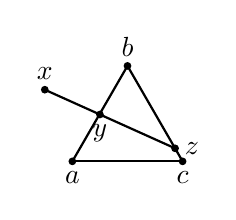
\begin{tikzpicture}[scale=0.7]
                % Draw the lines
                \draw[thick] (-1,0) -- (0,1.732);% node[right] {$L_1$};
                \draw[thick] (1,0) -- (0,1.732);% node[right] {$L_2$};
                \draw[thick] (-1,0) -- (1,0);
                % Draw the intersection point
                \fill (-1,0) circle (2pt) node[below] {$a$};
                \fill (0,1.732) circle (2pt) node[above] {$b$};
                \fill (1,0) circle (2pt) node[below] {$c$};

                \fill (-1.5,1.3) circle (2pt) node[above] {$x$};
                \fill (-0.5,0.85) circle (2pt) node[below] {$y$};
                \fill (0.86346, 0.23644) circle (2pt) node[right] {$z$};
                \draw[thick] (-1.5,1.3) -- (0.86346, 0.23644);
            \end{tikzpicture}
            \caption{Intuitively, regardless of our choice of $x$, since $xy$ also intersects $bc$, and $ac$, we'll have a distinct point $z$ on one of the two lines.}
        \end{figure}

        Suppose $y = z_1 = z_2$, then we have that all three lines $ab,bc,ac$ share one point $y$,
        but then $\{b, y\} \subseteq ab$ and $\{b, y\} \subseteq bc$, so $ab = by = bc$ by A1,
        since $by$ is the unique line passing through $b, y$.
        But this contradicts $ab, bc$ being distinct lines.
        Thus, we must have that $y \neq z$ where $z$ is one of $z_1$ or $z_2$.

        Finally, the line $xy$ contains points $y,z \in X_2$, and since $X_2$ is a subspace we must have that $xy \in X_2$
        So $X_2$ = $P$ since any two points in $P$ form a line (containing them) that is fully contained in $X_2$.
        Thus, the dimension is at most 2.
    \end{proof}

    This proof highlights the idea behind this geometric dimension definition,
    our chain of subspaces is akin to talking about different objects of increasing dimension in our space.
    That is, points in lines, lines in planes \ldots up to $n-1$ dimensional hyperplanes, to the full space itself.

    \section{Future Developments}

    As it turns out, order and dimension are powerful tools for classifying finite geometries.
    In fact, we use the notation $PG(n, q)$ to talk about finite projective spaces of dimension $n$ and order $q+1$
    that arise from a finite field of order $q$, written $GF(q)$ (since they are isomorphic up to order.)\cite[p.~xv]{hirschfeld_general_2016}

    The Veblen-Young theorem shows finite projective spaces of dimension $n \geq 3$ can always be described using such a field.
    However, finite projective planes are much harder to classify, since they can be constructed in more ways.
    Specifically, planes that do not satisfy the theorem of Desargues.\cite[\S3]{beutelspacher_projective_1998}

    The difficulty in classifying finite projective planes gives rise to an open conjecture:
    \textit{The order of a finite projective plane is always a prime power.}
    The number of non-isomorphic finite projective planes is only known up to order 10: $1, 1, 1, 1, 0, 1, 1, 4, 0$
    due to the computational complexity of verifying this using brute force\cite{lam_computer_1991,lam_non-existence_1989}.
    The closest we have come to a proof of this conjecture is the Bruck-Ryser theorem\cite[p.~26]{beutelspacher_projective_1998} which states if for positive integer $n$,
    $n \equiv 1,2\ (mod\ 4)$ and $n$ is not the sum of two squares, then no plane exists of order $n$.

    % References
    \newpage
    \bibliography{references}
    \bibliographystyle{IEEEtran}
\end{document}
